\documentclass{standalone}
\usepackage{tikz}
\usepackage{pgfplots}
\usepackage{filecontents}

\usetikzlibrary{decorations.pathreplacing,calc}

\newcommand{\tikzmark}[1]{\tikz[overlay,remember picture] \node (#1) {};}

% Generate PODModes.dat file

\begin{filecontents}{PODModes.dat}
	x    mode_1 mode_2 mode_3 
	-1 -0 -0 -0
   -0.875 -75.777237599909654 -1.4013162787009557 -1.4013162787009557
   -0.75 -144.65196201935416 -2.6797358555237967 -2.6797358555237967
   -0.625 -205.991147692247 -3.8230453359896956 -3.8230453359896956
   -0.5 -259.05759070726623 -4.8169286948791328 -4.8169286948791328
   -0.375 -303.02306440854574 -5.6452055794033749 -5.6452055794033749
   -0.25 -337.00284960177419 -6.2904745922901766 -6.2904745922901766
   -0.125 -360.11414712602948 -6.7352104912479671 -6.7352104912479671
   0 -371.55097337484091 -6.9631766682080585 -6.9631766682080585
   0.125 -370.65618340362448 -6.96078679819139 -6.96078679819139
   0.25 -356.96655620409615 -6.7179583305848478 -6.7179583305848478
   0.375 -330.21651849925053 -6.2281816633437268 -6.2281816633437268
   0.5 -290.30497074324506 -5.4878873151459944 -5.4878873151459944
   0.625 -237.24371794536205 -4.4954617326187121 -4.4954617326187121
   0.75 -171.10693228977922 -3.2502817499193739 -3.2502817499193739
   0.875 -91.992852374641956 -1.7519820647158324 -1.7519820647158324
   1 0 0 0
\end{filecontents}


\begin{document}
\pgfplotstableread{PODModes.dat}{\PODModes}

\begin{tikzpicture}
    [ bar/.style={black,draw=black, fill=black, fill opacity=1},
      dashedBar/.style={black,draw=black, fill=black, fill opacity=1, dashed},
      grid/.style={very thin, black, draw=gray!75},
      axis/.style={black,->,>=latex, thin},
      load/.style={black,fill=gray!70, fill opacity=0.4},
      dim/.style={latex-latex}]
      
  \scriptsize%


%%%%%%%%%%%%%%%%%%%%%%%%%%%%%%%%%%%%%%%%%%%%%%%%%%%%%%%%%%%%%%%%%%%%%%%%%%%%%%%%%%%%%%%%%%%%%%%%%%%%%%%%%%
%draw first layer discretization
	  
 % draw BSpline base mesh 
\node at(0,0) {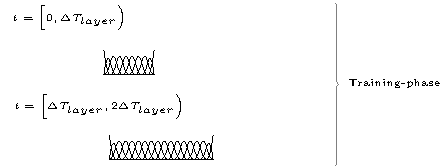
\includegraphics[width=1.05\textwidth]{TrainingPhaseScheme.pdf}};

 		
%%%%%%%%%%%%%%%%%%%%%%%%%%%%%%%%%%%%%%%%%%%%%%%%%%%%%%%%%%%%%%%%%%%%%%%%%%%%%%%%%%%%%%%%%%%%%%%%%%%%%%%%%%

 % draw Enriched mesh 
\node at(0,-6) {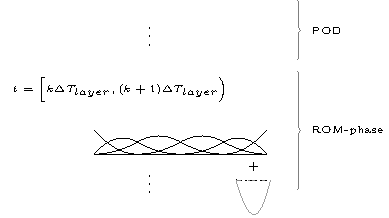
\includegraphics[width=\textwidth]{ROMPhaseScheme.pdf}};

 			
 		  
\end{tikzpicture}
\end{document}